\chapter{A No-Hair Test with a Free Quadrupole}
\label{ch:nohair}

\section{The Hartle--Thorne / quasi-Kerr metric}
\label{sec:ht}

To parametrise departures from Kerr we use the quasi-Kerr form of the
Hartle--Thorne metric \citep{HartleThorne1968,GlampedakisBabak2006}: the
total quadrupole is written
\begin{equation}
Q_{\rm tot} = -M a^2 + \epsq M^3,
\label{eq:qtot}
\end{equation}
and the deviation enters as a perturbation $h^{ab}$ of the \emph{inverse}
metric, valid through $\mathcal{O}(a^2,\epsq)$. At $\epsq = 0$ the
implementation reproduces the Kerr tensor to $10^{-12}$ (a dedicated unit
test), and for $\epsq \neq 0$ it produces the expected additional
pericentre advance $\delta\omega_Q = -3\pi\epsq\,(M/p)^2$ per orbit for
equatorial orbits of semilatus rectum $p$ \citep{Will2008}, which anchors
the sign convention of the perturbation. Because the far-field expansion of
the two structure functions $F_1, F_2$ of \citet{GlampedakisBabak2006}
suffers catastrophic cancellation at large $r$, the implementation
(\texttt{physics/src/hartle\_thorne.cpp}) switches
to an asymptotic series beyond $r = 9M$.

\stub{Geroch--Hansen multipole moments and the no-hair statement; the
Hartle--Thorne slow-rotation metric to $\mathcal{O}(a^2)$; the
$F_1, F_2$ structure functions and their large-$r$ cancellation, with the
branch-continuity test at the $9M$ switch.}

\section{Profile-likelihood constraint from S2}
\label{sec:nohairresult}

Re-fitting the S2 data in the free-quadrupole Hartle--Thorne spacetime
with $\epsq$ as a fourteenth parameter uses a
profile likelihood: $\epsq$ is stepped over a grid, the remaining
thirteen parameters are re-optimised at each step
(\texttt{OrbitFitter::fit\_nohair}), and
$\Delta\chi^2(\epsq) = \chi^2(\epsq) - \chi^2_{\rm min}$ is interpolated
to the $\Delta\chi^2 = 1$ (68 per cent) and $3.84$ (95 per cent)
crossings. The profile is flat at its Kerr value near $\epsq = 0$
(Fig.~\ref{fig:nohair}): the best fit is
$\epsq = \EpsQBest\times10^{5}$ with
$\sigma(\epsq) = \EpsQSigma\times10^{5}$ and a 95 per cent confidence
half-width of $\EpsQCiNinetyFive\times10^{5}$. The data are fully
consistent with the no-hair value $\epsq = 0$, and the marginal
$\chi^2_\nu$ is unchanged from the Kerr fit --- the extra degree of
freedom buys no improvement, as expected if Kerr is the true spacetime.

\begin{figure}
\centering
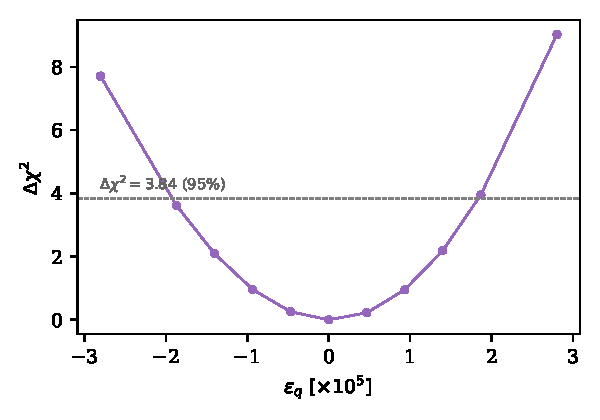
\includegraphics[width=0.7\textwidth]{figures/fig_nohair_profile.pdf}
\caption{$\Delta\chi^2$ profile of the quadrupole deviation $\epsq$ from
the S2 data. The 95 per cent interval is
$|\epsq| < \EpsQCiNinetyFive\times10^{5}$, consistent with the Kerr value
$\epsq = 0$.}
\label{fig:nohair}
\end{figure}

\section{Why the constraint is weak, and how it improves}
\label{sec:nohairforecast}

The constraint is weak in absolute terms because the quadrupole
pericentre shift scales as
$\delta\omega_Q = -3\pi\,\epsq\,(M/p)^2$ per orbit \citep{Will2008}.
Working the numbers: $M/p = R_g/p = 0.0424/228 = 1.86\times10^{-4}$, so
$(M/p)^2 = 3.5\times10^{-8}$ and one unit of $\epsq$ moves the pericentre
by only $3.3\times10^{-7}$~rad per orbit --- $0.07$~arcsec, versus an
astrometric sensitivity to $\omega$ of order $0.5\degr$ per orbit
(Table~\ref{tab:fit}). Inverting, the expected $1\sigma$ reach is
$\sigma(\epsq) \sim (0.5\degr)/(0.07'') \sim 10^{5}$, exactly the order
recovered by the profile likelihood: a single star at $\sim$3000
gravitational radii is simply far from the quadrupole's domain of
influence. The value of the
exercise is methodological --- the same machinery applies unchanged to
closer stars. Continued monitoring helps too: propagating the fitted
covariance forward, ten further S2 orbits (astrometry and RV of the
quality of the existing series) shrink the uncertainty to
$\sigma(\epsq) \approx \EpsQForecastTenOrbits\times10^{5}$, a factor
$\sim$3. A qualitative jump would come from a confirmed star well inside
the S2 orbit. The reported candidate S62, with a claimed 9.9-yr period and
$\sim$36~au pericentre, would be such a star, but we emphasise:
\emph{S62 is a contested orbit --- its identification is unconfirmed and
may be a misidentification of S29 or a blend artefact}; we therefore do
not build quantitative forecasts on it, and any future use of S62 in this
context must carry the same caveat.

\stub{New figures: $(M, \epsq)$ and $(\epsq, \astar)$ confidence contours
(needs the MCMC chains of Chapter~\ref{ch:fitting}); the no-hair corner
plot.}
